\chapter{Systemkrav}\label{Systemkrav}
\section{Systembeskrivelse}
Automatisk Ultralydsscanner er et system, som gør det muligt at lave en automatiseret ultralydscanning af mamma mhp. screning for brystkræft. Systemet Automatisk Ultralydsscanner består af en robotarm, en PC Applikation med en grafisk brugergrænseflade (GUI), et 3D kamera og en ultralydsscanner. Se figur \ref{Systembeskrivelse} nedenfor. 

Via GUI kan en operatør med kendskab til ultralyd interagere med systemet. Operatøren udfører først en 3D scanning af brystet, hvorefter systemet leverer information om brystområdets form og position fra 3D kameraet til robotarmen. Derefter kan mammografiscranningen foretages, hvor robotarmen med påmonteret ultralydsscanner fører ultralydsproben fra ultralydsscanneren rundt på det detekterede brystområdet. Ultralydsscanningen vises på ultralydsscannerens skærm, hvor operatøren kan følge med under scanningen.

Figuren nedenfor viser en oversigt over, hvordan elementerne i Automatisk Ultralydsscanner integrerer med hinanden.
 
\begin{figure}[H]
    \centering
    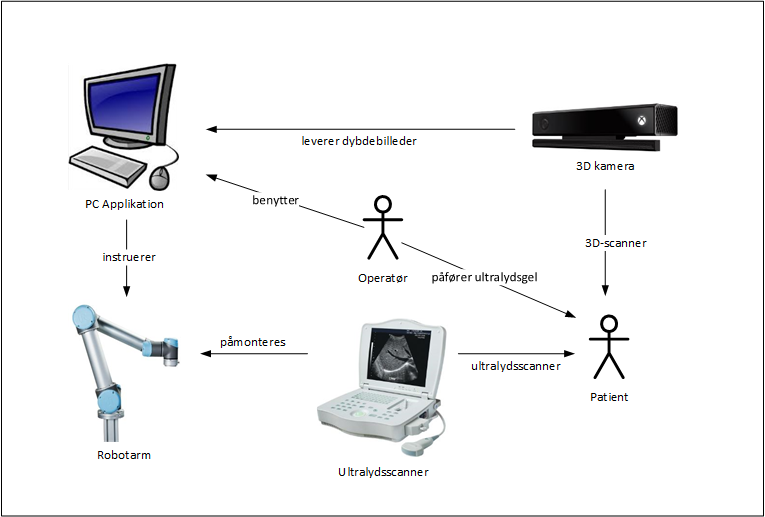
\includegraphics[width=0.75\textwidth]{figurer/d/Kravspecifikation/Systembeskrivelse}
    \caption{Systemoversigt over Automatisk Ultralydsscanner, der beskriver systemets opbygning og hvorledes de enkelte elementer interagerer}
    \label{Systembeskrivelse}
\end{figure}

\section{Aktører}
Der er indentificeret fem aktører, som integerer med systemet. Aktørerne inkluderer en operatør, patient, robotarm, ultralydsscanner og et 3D kamera. Operatør betjener systemet, mens scanningen foregår på patienten. 3D kameraet afgrænser området, der skal scannes, mens robotarm styrer en påmonteret ultralydsscanner i et specifikt overlappende bevægelsesmønster på det detekterede område.

\section{Funktionelle krav}
De funktionelle krav for Automatisk Ultralydsscanner er defineret ved brug af use cases (UC). Til systemet er der identificeret fire use cases, som kan ses i use case diagrammet på Figur \ref{UseCaseDiagram} 

Operatøren gør klar til scranning ved at opstarte system (UC1: Start System). Hovedmenuen på GUI vil vises, hvorpå operatøren kan vælge at 3D scanne patientens brystområde (UC2: 3D scan brystområde). Inden der kan ultralydsscannes, skal operatøren påføre en gel for en bedre scanning. Operatøren har mulighed for at vælge at lave en ultralydsscanning på GUI, hvorefter robotarmen vil køre over brystet (UC3: Ultrascan brystområde).  Operatøren kan derefter på GUI vælge at stoppe systemet (UC4: Stop System). 

\begin{figure}[H]
    \centering
    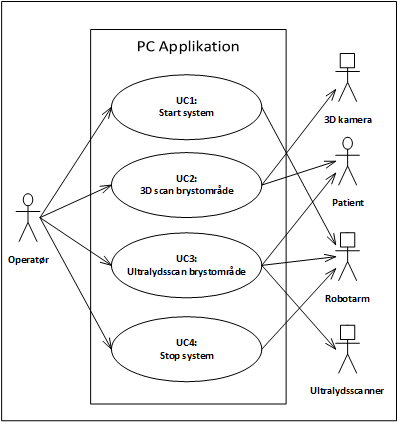
\includegraphics[width=0.75\textwidth]{figurer/d/Kravspecifikation/UseCaseDiagram}
    \caption{Use case diagram for Automatisk Ultralydsscanner, der viser systemets funktionaliteter og aktørernes relation hertil.}
    \label{UseCaseDiagram}
\end{figure}

\section{Ikke-funktionelle krav}
De ikke-funktionelle krav for Automatisk Ultralydsscanner er beskrevet ved brug af MoSCoW og FURPS+. Det er kun must-krav der er implementeret og specielt performancestider for Automatisk Ultralydsscanners er prioriteret, for at systemet kan udføre en scanning på samme tid som en radiolog. Nedenfor kan de implementerede ikke-funktionelle krav ses. 

\subsubsection{Usability}
\begin{itemize}
    \item [U1.] PC Applikation skal have en GUI. (must)
     \item[U2.] GUI skal have en procent-indikator for ultralydsscanningens gennemløb. (must)
\end{itemize}

\subsubsection{Performance}
\begin{itemize}
    \item[P1.] Scaningen med 3D kamera og ultralydsscanning skal max tage 10 minutter til sammen. (must) 
    \item[P2.] Starttid på PC Applikation skal være max 10 sekunder. (must)
    \item[P3.] 3D kamera skal max bruge 10 sekunder på at tage 3D billedet. (must)
    \item[P4.] PC Applikation skal max 10 sekunder på at færdiggøre brystområdets positurer til Robotarm. (must)
\end{itemize}

\subsection{Ekstra}
Lovkravene til medicinsk udstyr og software til medicinske udstyr, burde have været en must-krav i de ikke-funktionelle krav til Automatisk Ultralydsscanner, men da den medicinske godkendelse først blev udarbejdet sent i udviklingsprocessen er kravene fra den medicinske godkendelse ikke implementeret i systemet. Dette er for eksempel krav som at Autoamtisk Ultralydsscanner skal: 

\begin{itemize}
\item Designes så det ikke er til fare for bruger om patient. 
\item Fremstilles i et materiale som mindsker spredning af bakterier. 
\item Have tydelige og letforståelige tegn på knapper og display.
\item Have et risikohåndteringssystem
\item Have kvalitetssikringssystem. 
\item Mærkes så der ikke kan være tvivl om hvordan produktet skal bruges.
\item Kunne modstå en luftbåren ESD-transient på op til ±8 kiloVolt
\item Kunne tåle en indstråling på 3V/m
\end{itemize}